\section{Metodologia}%
\label{sec:metodologia}

Para a condução deste trabalho, foi realizada uma pesquisa bibliográfica sobre o problema, incluindo a natureza das restrições e os limites superiores e inferiores possíveis para suas variáveis~\cite{HEIDARI2019849}.

\subsection{Função Objetivo}

Com base em \citeonline{fauzi_truss}, compreendemos que o problema envolve a minimização da área da seção transversal das três barras que compõem uma treliça. Para evitar que o problema se torne multiobjetivo, a avaliação é feita considerando um peso fixo hipotético posicionado sobre a treliça, de forma que o único objetivo é minimizar o peso total da estrutura, mantendo sua capacidade de suportar tal peso.

Assim, seções transversais menores resultam em um peso menor e, consequentemente, em uma solução de melhor qualidade. Embora à primeira vista o problema pareça requerer três variáveis (uma para cada barra da treliça), a simetria estrutural exige que as barras diagonais tenham seções iguais, evitando tendências de giro que poderiam comprometer a integridade da estrutura.
Tal propriedade pode ser visualizada na \autoref{fig:f1}, em que a barra 2 é horizontal e as barras 1 e 3 são diagonais.

Dessa forma, as barras 1 e 3 devem ter a mesma área de seção transversal, reduzindo o problema para duas variáveis, quais sejam:
\begin{symbols}
    \item[\(x_1\) Área da seção transversal das barras 1 e 3]
    \item[\(x_2\) Área da seção transversal da barra 2]
\end{symbols}

\begin{figure}[!ht]%
    \centering
    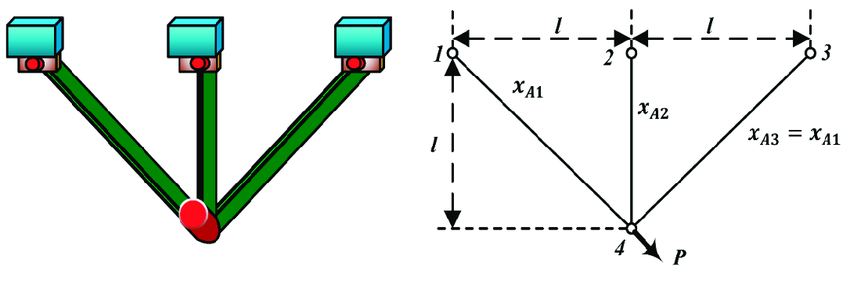
\includegraphics[scale=1]{images/Three-Bar-Truss-Design.png}
    \caption{Representação do \gls{problem}. Fonte: \citeonline{fauzi_truss}.}%
    \label{fig:f1}
\end{figure}

A função objetivo pode ser expressa como:

\begin{equation}
    \begin{split}
        y = \left( 2 \sqrt{2} \cdot x_1 + x_2 \right) \cdot l \\
        \text{onde~}
        0 \leq x_1, x_2 \leq 1 \text{~e~}
        l = 100 \text{~cm}.
    \end{split}
\end{equation}

\subsection{Restrições}

O problema está sujeito a restrições de tensão, deflexão e flambagem~\cite{fauzi_truss}, com um valor máximo permitido de 2 em todos os casos.
Se \(g_x > 0\), ocorre uma violação da restrição, o que significa que a solução proposta não é viável estruturalmente.
As restrições são expressas pelas seguintes equações:

\begin{gather}
    \begin{subequations}
        \begin{align}
            \begin{split}
                g_1 = \frac{2 \left( \sqrt{2} \cdot x_1 + x_2 \right)}{\sqrt{2} \cdot x_1^2 + 2 \cdot x_1 \cdot x_2} - 2
            \end{split}
            \\
            \begin{split}
                g_2 = \frac{2 \cdot x_2}{\sqrt{2} \cdot x_1^2 + 2 \cdot x_1 \cdot x_2} - 2
            \end{split}
            \\
            \begin{split}
                g_3 = \frac{2}{x_1 + \sqrt{2} \cdot x_2} - 2
            \end{split}
        \end{align}
    \end{subequations}
\end{gather}
\begin{equation*}
    \begin{aligned}
        \text{onde~}
        0 \leq x_1, x_2 \leq 1, \\
        P = 2 \text{~KN/cm}^2,  \\
        \sigma = 2 \text{~KN/cm}^2.
    \end{aligned}
\end{equation*}

\subsection{Penalização}

Caso alguma das restrições \(g_1\), \(g_2\) ou \(g_3\) seja positiva, a restrição será violada, indicando que a solução é estruturalmente inviável.
Para esses casos, são estabelecidos dois valores de penalização:\(\phi \) e \(\text{viol}\), que são adicionados à função objetivo.
Esses valores positivos prejudicam a qualidade da solução, dado que se trata de uma função de minimização.

O valor \(\phi \) é a soma dos valores que violam as restrições, enquanto \(\text{viol}\) representa o número de restrições violadas.

\begin{gather}
    \begin{align}
        \begin{split}
            \phi = \sum \max(g_i, 0) \\
            \text{onde~} i = 1, 2, 3
        \end{split}
    \end{align}
\end{gather}


\subsubsection{Função Objetivo Penalizada}

A função objetivo penalizada é dada por:
\begin{gather}
    \begin{align}
        \begin{split}
            f(x) = y + w_1 \cdot \phi + w_2 \cdot \text{viol}
        \end{split}
    \end{align}
\end{gather}

Cujos componentes são:

\begin{symbols}
    \item[\(f(x)\)] Função objetivo penalizada
    \item[\(y\)] Função objetivo
    \item[\(w_i\)] Peso associado à penalização por violação
    \item[\(\phi s\)] Valor de penalização
    \item[\(\text{viol}\)] Número de restrições violadas
\end{symbols}

\subsection{Configuração dos Experimentos}

A seguir, apresentamos as constantes e parâmetros selecionados para a realização dos experimentos.

\subsubsection{Constantes}

As constantes utilizadas em ambos os experimentos estão listadas na \autoref{tab:constantes-comuns}.

\begin{table}[htb]
    \center%
    \begin{tabular}{l l}
        \bottomrule
        \textbf{Constante}   & \textbf{Valor} \\ \midrule
        Direção              & Min            \\ \midrule
        Tamanho da população & 50             \\ \midrule
        Tipo de seleção      & Torneio        \\ \midrule
        População no torneio & 20\%           \\
        \midrule
        Mutação              & Flip           \\ \midrule
    \end{tabular}
    \caption{Constantes utilizadas am ambos os experimentos.}%
    \label{tab:constantes-comuns}
\end{table}

As constantes utilizadas no experimento do algoritmo genético estão listadas na \autoref{tab:constantes-genetico}.
Destacam-se como específicas o tamanho da população a ser mantida entre duas gerações, tanto considerando os melhores indivíduos e os piores.

\begin{table}[htb]
    \center%
    \begin{tabular}{l l}
        \bottomrule
        \textbf{Constante}  & \textbf{Valor} \\ \midrule
        Tipo de crossover   & Aritmético     \\ \midrule
        Taxa de crossover   & 90\%           \\ \midrule
        Taxa de mutação     & 5\%            \\ \midrule
        Elitismo (melhores) & 10\%           \\ \midrule
        Elitismo (piores)   & 30\%           \\ \midrule
        Gerações            & 1500           \\ \toprule
    \end{tabular}
    \caption{Constantes utilizadas no experimento com o \gls{esga}.}%
    \label{tab:constantes-genetico}
\end{table}

\begin{table}[htb]
    \center%
    \begin{tabular}{l l}
        \bottomrule
        \textbf{Constante}       & \textbf{Valor} \\ \midrule
        Tipo de crossover        & Um ponto       \\ \midrule
        Taxa de crossover        & 85\%           \\ \midrule
        Taxa de mutação          & 15\%           \\ \midrule
        Taxa de exploração local & 0.5            \\ \midrule
        Máx. gerações locais     & 10             \\ \midrule
        Bits por parâmetro       & 4              \\ \midrule
        Gerações                 & 100            \\ \toprule
    \end{tabular}
    \caption{Constantes utilizadas no experimento com o \gls{oma}.}%
    \label{tab:constantes-memetico}
\end{table}

O algoritmo memético, por ser uma extensão do algoritmo genético, utiliza parâmetros similares, como mostrado na \autoref{tab:constantes-memetico}, variando apenas o tipo e a taxa de \gls{crossover}, a taxa de mutação e o número de gerações, além dos parâmetros específicos.
São eles a taxa de exploração utilizada pelo resolvedor local integrado, o número máximo de gerações locais e o número de bits por parâmetro, que determina a precisão da codificação.

As variáveis de decisão, \(x_1\) e \(x_2\), que representam as áreas das seções transversais das barras, foram normalizadas para o intervalo de 0 a 1, garantindo consistência na avaliação dos resultados. A população inicial é gerada aleatoriamente dentro desse intervalo, e seu tamanho permanece fixo em 50 indivíduos ao longo de todas as gerações.

O operador de \gls{crossover} é aplicado com uma taxa de 90\%. A mutação, com uma taxa de 5\%, é realizada utilizando o método \texttt{flip}. O elitismo é aplicado a 10\% dos melhores indivíduos e a 30\% dos piores. No algoritmo genético, a execução ocorre por 1500 gerações, enquanto no algoritmo memético, por 100 gerações.

\subsection{Parâmetros e Variáveis}

Os experimentos foram conduzidos utilizando os parâmetros que apresentaram os melhores resultados nas etapas anteriores deste trabalho. Assim, a única parametrização dinâmica do experimento, isto é, o parâmetro que varia entre as execuções, foram os pesos atribuídos a cada tipo de penalização.

Para garantir a robustez dos resultados, os experimentos foram repetidos 10 vezes para cada algoritmo, utilizando \textit{seeds} diferentes para a geração de números aleatórios.